%% Label Bias and Environmental Datashift
\chapter{Label Bias and Environmental Datashift}
\label{chap:chap3}
\section*{Label Bias}
Bias is the result of inadequate data where a certain group or class is favoured over another/others hence creating an overrepresentation \cite{Jiang}\cite{saria2019tutorial}.
ML models trained using such datasets will acquire these underlying biases hence making incorrect predictions.

The following mathematical framework, developed by researchers at Google, can be used as a representation to undestand bias in data \cite{Jiang}.

% \begin{figure}[h]
%     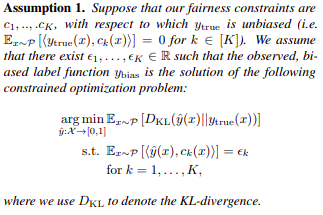
\includegraphics[scale =0.8]{Assumption.png}
%     \centering
%     \caption{Bias Assumption \cite{Jiang}}
%     \label{fig:Assumption}
% \end{figure}
\bigskip
\begin{center}
    \begin{tabular}{l}
        \textbf{Assumption 1: }Presume fairness constraints are $c_1, ..., c_K$,\\
        where $y_{true}$ is biased, namely $\EX_{x\sim p}[\langle y_{true}(x), c_k(x)\rangle] = 0$ for $k \in [K]$\\
        Assuming that $\in_1, ..., \in_k \in \R$ exists and the observed biased label \\
        function, $y_{bias}$ is the solution of the following equation.
    \end{tabular}

    \begin{equation}
        \label{eq:assumption}
        \begin{split}
            & \underset{\hat{y}:\chi\rightarrow[0,1]}{\text{arg min}}  \EX_{x\sim P}[D_{KL}(\hat{y}(x)||y_{true}(x))]\\
            & \text{s.t} \EX_{x\sim P}[\langle\hat{y}(x),c_k(x)\rangle] = \in_k \\
            & \text{for } k = 1, ..., K.
        \end{split}
    \end{equation}
    $D_{KL}$ signifies KL-divergence
\end{center}

\bigskip
In figure (\ref{eq:assumption}), the assumption is that $y_{bias}$ is the label which is closest to $y_{true}$ and achieves a measure of bias.
In cases where data has been manually manipulated by human input, either consciously or subconsciously, this is deemed to be a reasonable assumption.
The contiguity to $y_{true}$ is given by the KL-divergance, which is used to establish the notion of accurate labeling. 
The Proposition in figure (\ref{eq:Proposition}) is derived from the KL-divergence. (For complete proof of proposition, see \cite{Jiang})
\enlargethispage{-2\baselineskip}
% \begin{figure}[h]
%     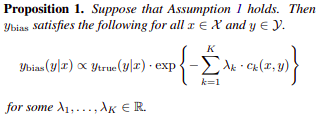
\includegraphics[scale =0.8]{Prop.png}
%     \centering
%     \caption{Bias Proposition \cite{Jiang}}
%     \label{fig:Proposition}
% \end{figure}

\bigskip
\begin{center}
    \begin{tabular}{l}
        \textbf{Proposition 1: } Presume Assumption 1 holds, \\
        $y_{bias}$ satisfies the following equation (for $x \in \chi \text{ and } y \in y$) \\
    \end{tabular}

    \begin{equation}
        \label{eq:Proposition}
        \begin{split}
            & y_{bias}(y|x) \text{ }\alpha \text{ } y_{true}(y|x) \cdot \text{exp} \Bigg\{ -\sum^K_{k=1} \lambda_k \cdot c_k(x,y)\Bigg\} \\
            & \textit{for some } \lambda_1, ..., \lambda_K \in \R
        \end{split}
    \end{equation}
\end{center}

\bigskip
Now that $y_{bias}$ is represented in terms of $y_{true}$, we can infer $y_{true}$ in terms of $y_{bias}$ as represented in Figure (\ref{eq:Corollary}).

% \begin{figure}[h]
%     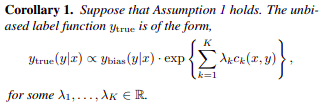
\includegraphics[scale =0.8]{corollary.png}
%     \centering
%     \caption{Bias Corollary \cite{Jiang}}
%     \label{fig:Corollary}
% \end{figure}

\bigskip
\begin{center}
    \begin{tabular}{l}
        \textbf{Corollary 1: } Presume Assumption 1 still holds. \\
        The unbiased label function, $y_{bias}$ is nor represented as:
    \end{tabular}

    \begin{equation}
        \label{eq:Corollary}
        \begin{split}
            & y_{true}(y|x) \text{ }\alpha \text{ } y_{bias}(y|x) \cdot \text{exp} \Bigg\{ \sum^K_{k=1} \lambda_k \cdot c_k(x,y)\Bigg\} \\
            & \textit{for some } \lambda_1, ..., \lambda_K \in \R
        \end{split}
    \end{equation}
\end{center}

\section*{Datashift}
There may be situations where performance issues may not be apparent during training stages. 
They instead appear post-deployment where training and deployment datasets can have irregularities. 
This is known as Environmental Datashift \cite{saria2019tutorial}. 
This calls into question whether the ML model is robust enough to generalise well to new samples beyond training, or whether it tends to over-generalise to the training dataset thus resulting in unreliability in the real world.

In \cite{shift}, datashift has been mathematically modelled in two scenarios as follows:

Assuming classifier, $\mathcal{F}$ has been fairly trained with true labels, $Z$, at $t = 0$ (where $t = 0$ signifies time of training and $t = 1$). signifies a new timestep).
Parameters such as binary classification and probability of privelaged and distadvantaged class, $\zeta_A$,  $\zeta_B$, $\rho_A$ and $\rho_B$ respectively,
may change from  $t = 0$ to $t = 1$.

The first scenario being when there is no access to the new labels at $t = 1$. 
Therefore the structure of the bias model at $t = 1$ is not apparent, but $Z$ has changed.
Consequently, $\zeta_A \text{ and } \zeta_B$ have also changed. 
We can assume:
\begin{align*}
    \text{label shift: } & P(B)_{t=0} = P(B)_{t=1} \\
    \text{covariate shift: } & P(B)_{t=0} \neq P(B)_{t=1}
\end{align*}

The second scenario is when there is access to the new biased labels, 
in cases where deployment environment data is collected to validate the bias model at $t = 1$.
There are two viable causes for shift, true distribution changes and bias model changes.

True distribution changes are alike to the first scenario where distribution, $\mathcal{D}_{t=1} \neq \mathcal{D}_{t=0}$.
In bias model changes, the true distribution labels may be the same but label shift has occured as a result of changing $\mathcal{G}$.
This also means probability, $p_A$ and/or $p_B$ could have also changed resulting in concept shift.


\section{Dataset \& Preprocessing}
The predictive maintenance dataset \cite{ahonen} will be used to model bias and environmental datashift while classifying failures of an ioT gadget/s.
During one week, maintenance data was collected from six devices every hour for 168 hrs.
Therefore, this data set contains 1008 rows of data. 
Each cycle of data reading contains the following measurements: 

\begin{table}[H]
    \begin{center}
        \caption{Measurements Dataset} 
        \begin{tabular}{ ll } 
         \toprule
         \textbf{Measurement} & \textbf{Description} \\  [0.5ex] 
         \midrule
         \textbf{Measurement Time} & Time \\
         \textbf{Gadget ID} & Device number \\
         \textbf{Vibration x sensor} & Horizontal vibration \\ 
         \textbf{Vibration y sensor} & Vertical vibration \\ 
         \textbf{Pressure sensor} & Hose pressure \\
         \textbf{Temperature sensor} & Internal temperature \\
         \bottomrule
        \end{tabular}
    \end{center}
\end{table}

The failures dataset contains the precise times each gadget failed. 
During the course of the week, 105 failures were recorded. 
The two datasets were combined and additional labels were added (\ref{table:labels}) for use in training and prediction.
The model was trained using \textit{'Vibration y'}, \textit{'Temperature 6hr Std'}, 
and \textit{'Pressure 6hr Mean'} as feature labels, and predictions were tested using class label, \textit{'Fail in 1hr'},
where positive classification of device failure occurs when the time remaining to device failure is less than one hour.

\begin{table}[H]
    \begin{center}
        \caption{Maniupulated data labels}
        \label{table:labels} 
        \begin{tabular}{ll}
            \toprule
            \textbf{Labels} & \textbf{Description} \\ [0.5ex]
            \midrule
            \textbf{Temperature 6hr Std} & Standard Deviation of last 6 measurements \\
            \textbf{Pressure 6hr Mean} & Average of last 6 measurements \\
            \textbf{Fail in 1hr} & If failure will occur within the next hour \\
            \bottomrule
        \end{tabular}
    \end{center}
\end{table}

The complete dataset was then split 70-30\% for training and testing respectively. 
In addition, the train dataset was split into two further datasets, DF1 and DF2. 
DF1 contained all data from devices with 'Gadget ID' 1,2 and 3 while DF2 contained all data from devices with 'Gadget ID' 3,4 and 5.
Concsequently, the test dataset was also split into 'Sample 1' and 'Sample 2' in the same manner as DF1 and DF2.

\begin{table}[H]
    \begin{center}
        \caption{Training and Testing Datasets}
        \label{table:datasets} 
        \begin{tabular}{lll}
            \toprule
            \textbf{Dataset} & \textbf{Size} &\textbf{Description} \\ [0.5ex]
            \midrule
            \textbf{Full Train} &685& 70\% of the complete dataset. Used for training model \\
            \textbf{Full Test}  &293& 30\% of the complete dataset. Used for testing model \\
            \textbf{DF1}        &339& Only samples from \textbf{Full Train} with Gadget ID 1,2 \& 3 \\
            \textbf{DF2}        &346& Only samples from \textbf{Full Train} with Gadget ID 4,5 \& 6 \\
            \textbf{Sample 1}   &150& Only samples from \textbf{Full Test} with Gadget ID 1,2 \& 3 \\
            \textbf{Sample 2}   &145& Only samples from \textbf{Full Test} with Gadget ID 4,5 \& 6 \\
            \bottomrule
        \end{tabular}
    \end{center}
\end{table}

\section{Experimental Results}
It has previously been assumed that bias occurs when one type of sample is over represented over another/others.
By training a model with DF1 or DF2 dataset instead of the Full Train dataset, samples of certain devices have been completely overlooked and hence bias exists within DF1 and DF2. 
Using Table (\ref{table:Bias}), we can compare the metrics of Full Train, DF1 and DF2 sets when tested against the Full Test set.
Although DF1 improves amongst most metrics of the Full Test, we observe a deacrease in performance in the model trained with DF2.
The increase in metrics of DF1 may suggest higher importance of those samples over DF2 but it is difficult to be certain due to the small dataset size (under 1000 samples).

% \enlargethispage{5\baselineskip}
\bigskip
\begin{table}[H]
    \begin{center}
        \caption{PDM Label Bias and Environmental Datashift Evaluation Results - SVM}
        \label{table:Bias}
        \begin{tabular}{lccccccc}
            \toprule
            \multicolumn{1}{c}{\textbf{Metric}} & \multicolumn{7}{c}{\textbf{Datasets}}                                                                                                                                                                                                      \\ \midrule
            \multicolumn{1}{l}{}      & \multicolumn{1}{c|}{Full Train} & \multicolumn{3}{c|}{DF1}                                                                       & \multicolumn{3}{c}{DF2}                                                                       \\ \cline{2-8} 
            \multicolumn{1}{l}{}      & \multicolumn{1}{l|}{Full Test}  & \multicolumn{1}{l|}{Full Test} & \multicolumn{1}{l|}{Sample 1} & \multicolumn{1}{l|}{DF2} & \multicolumn{1}{l|}{Full Test} & \multicolumn{1}{l|}{Sample 2} & \multicolumn{1}{l}{DF1} \\ 
            \midrule
            \textbf{Accuracy}   & 0.778 &0.788  &0.816  &0.675  &0.775      &0.778  &0.743\\
            \textbf{Precision}  &0.91   &0.93   &0.93   &0.91   &0.91       &0.93   &0.91\\
            \textbf{Recall}     &0.78   &0.79   &0.82   &0.67   &0.77       &0.78   &0.74\\
            \textbf{F1 Score}   &0.82   &0.82   &0.85   &0.74   &0.81       &0.82   &0.79\\
            % \midrule
            \bottomrule
        \end{tabular}
    \end{center}
\end{table}

\enlargethispage{\baselineskip}
In the case of Environmental Datashift,\textit{
"modelers typically assume that training data
is representative of the target population or environment where
the model will be deployed" - \cite{saria2019tutorial}}
We take a scenario where a model is trained on dataset DF1.
Remembering DF1 and Sample 1 datasets are only concerned with samples from Gadgets 1, 2 \& 3, it is expected that this combination will offer the highest results.
Experimental results in Table (\ref{table:Bias}) and the plots in Figures (\ref{fig:DF1}) \& (\ref{fig:DF2}) back this claim. 
Moving further, testing the model with Full Test yields the next best results as it contains a mix of already seen and completely new samples.   
Performance is affected severely when the model is tested using DF2 as the samples have irregularities when compared to training data.
The same observations can be made when training the model on DF2 dataset.
This model is not robust enough to generalise to new samples and solutions are offered in subsequent sections. 

\begin{figure}[H]
    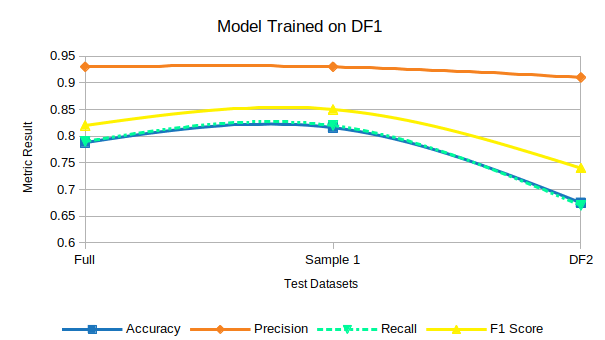
\includegraphics[scale =0.75]{Bias_DF1.png}
    \centering
    \caption{Test Datasets on DF1 metrics}
    \label{fig:DF1}
\end{figure}

\begin{figure}[H]
    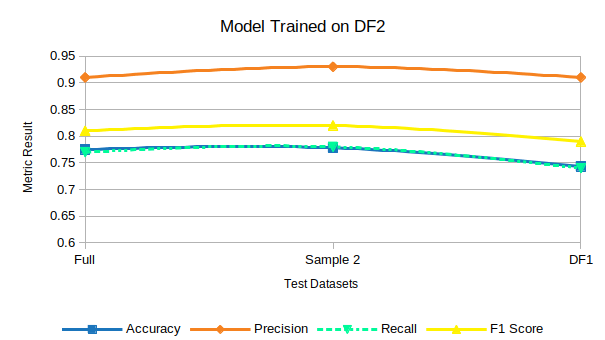
\includegraphics[scale =0.75]{Bias_DF2.png}
    \centering
    \caption{Test Datasets on DF2 metrics}
    \label{fig:DF2}
\end{figure}


% \hl{Consider noise in dataset due to uneccassry labels}

\section{Further Research}
Research performed in \cite{Jiang}, offers solutions to deal with biased datasets and compares these solutions across various datasets.
The following datasets were used in this experiment:
\begin{itemize}
    \item Bank Marketing - Prediction of subscription to bank product using age as the protected attribute
    \item Communities \& Crime - Determine wheter a community has a high crime rate. Four race features are used as protected attributes
    \item ProPublicas COMPAS - Predict recidivism based on a number of factors. Protected attributes are two race based and two gender biased
    \item German Statlog Credit Data - Predict good or bad credit rating. Two protected groups seperated by age.
    \item Adult Income - Predict if individual income is greater than \$50k. Two protected groups based on gender and another two groups based on race.
\end{itemize}

\enlargethispage{\baselineskip}
\begin{table}[H]
    \bigskip
    \caption{Benchmark Fairness Tests on Multiple Datasets \cite{Jiang}}
    \begin{figure}[H]
        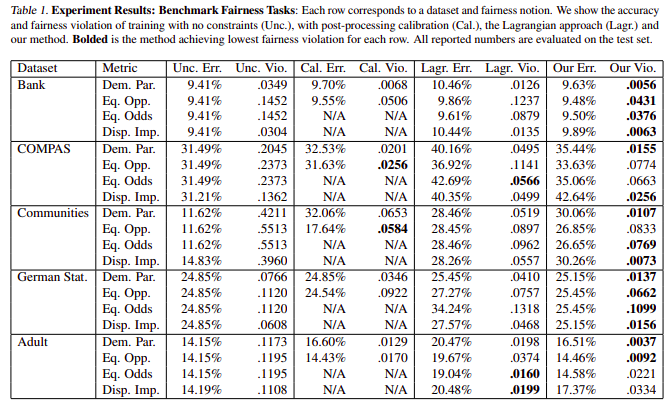
\includegraphics[scale=0.65]{label_bias.png}
        \centering
    \end{figure}
    \label{table:fairness}
\end{table}

As can be viewed in Table \ref{table:Bias} all models were trained initially without any attempt to solve the bias problem (Unc.).
Following on, Post-processing, Lagrangian Approach and a newly proposed method were applied and tested for fairness violation.
It is observed that implementation of all approaches increases fairness as the violation decreases when compared to Uncalibrated results.

\bigskip
A study carried out by Samsung Research \cite{8953715} performs experimentation on data bias and environmental datashift with Deep Neural Networks in a similar fashion to our own experiment in the previous section.

Bias was deliberately produced within three different datasets in this study investigate the algorithm's ability to unlearn bias. 
We are only concerned with the Dogs and Cats dataset and IMDB Face datasets.
The Dogs and Cats dataset consisted of 25,000 images which was then divided between TB1 and TB2 according to the colour of dogs/cats to produce bias as desired.
This method of segregation ensures any sample in TB2 will not be found in TB1 and vice-versa.
The Test dataset consisted 12,500 images. 

The IMDB Face dataset was also segregated in a similar manner.
The Test set accounted for 20\% of the entire dataset and the remaining was used for training.
EB1 and EB2 datasets were formed based on age and gender of actors. There was no common data samples between any of these datasets.

\begin{table}[H]
    % \bigskip
    \caption{Evaluation Results on Dogs and Cats Dataset \cite{8953715}}
    \begin{figure}[H]
        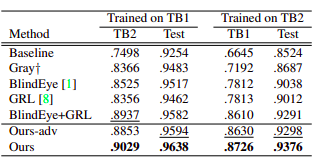
\includegraphics[scale=0.95]{samsung_TB.png}
        \centering
    \end{figure}
    \label{table:Dogs and Cats}
\end{table}

\begin{table}[H]
    % \bigskip
    \caption{Evaluation Results on IMDB Face Dataset \cite{8953715}}
    \begin{figure}[H]
        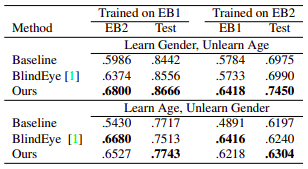
\includegraphics[scale =0.95]{Samsung_EB.png}
        \centering
    \end{figure}
    \label{table:IMDB}
\end{table}

By observing results presented in Tables (\ref{table:Dogs and Cats} \& \ref{table:IMDB}), the effects of environmental datashift become apparent.
When trained on TB1/EB1, networks tested on the full Test sets always perform better as the network is unable to generalise well enough to TB2/EB2.
However, the experiment also proves thats methods can be implemented to claw back some of the lost performance. 
Examining the Dogs and Cats dataset, the baseline result shows approximately 20\% reduction in performance on networks tested on TB1/2 when compared to the Test set.
All evaluated methods are able to improve the percentage difference between biased datasets and the Test set. 
The best method is able to bring the percentage difference down to approximately 5\%.

\pagebreak
\section{Recommendations}
\subsection{Pre-processing} 
When it comes to creating ML models for fair and unbiased predictions, the first area of investigation should be the data.
In \cite{saria2019tutorial} and accompanying material, the issue of inadequate data is presented where the limited availability of data on minor subsets creates negative bias towards that sub-population.
Issues of this nature arise when when the model is tested on the broader dataset where the resulting performance is rated highly and performance on individual subsets is not evaluated.
Therefore, it is important to measure performance on all sub-populations to determine and understand the true performance of the ML model.

Another method to diagnose and identify reliability concerns if the sub-pupulations of interest are initially unknown 
would be to cluster the input space into regions of high and low density.
In low density regions, we would then need to investigate the regions to identify any correlation with attributes of concern or importance.

In cases where the performance in any one of the sub-populations is not up to standard, the simple remedy to this issue would be to collect or use data which better represents sub-pupulations of interest.
This could be the use of more data, or use of more quality data in general.
Another solution is to try and modify the objective function to balance out the sub-populations. 
Therefore, the underperforming data is given a higher weight and/or decrease the wight of data which is overrepresented. 

When developing ML models which are invariant and are able to generalise well to shifts in data, 'reactive' solutions are predominantly offered.
This involves optimising the model for its intended environment by using unlabeled data samples from the target distribution.
This optimisation is usually carried out by implementing various techniques such as reweighting in order to adapt to the new deployment environment.
However, reactive methods are only useful when the actual environment data is available for investigation. 

In situations were we cannot anticipate this change in environment, proactive solutions are preferred.
Proactive solutions teach the model to protect from likely problematic shifts by forecasting possible shifts.
In \cite{subbaswamy2019preventing}, a framework is presented to teach predicitive models to 'transport' or adapt to dataset shift.
This framework uses directed acyclic graphs (DAGs) to represent how data shifts from unstable to stable environments in the data generation process (DGP).
Here $X$ are the inputs, and $T$ is prediction. The result, $T$ given $X$ is stable (doesn't change over time).
The selection variable, $S$ indicates what is likely to change. The use of DAGs assists in the identification of shifts which need to be protected against.

\begin{figure}[H]
    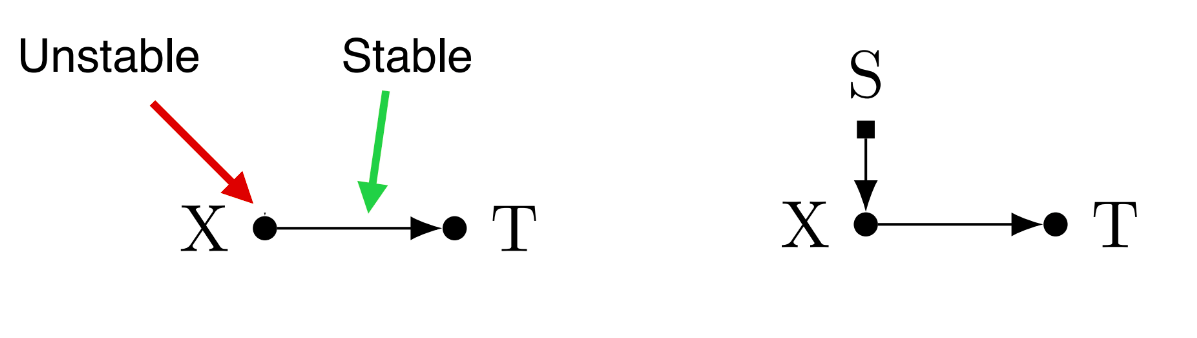
\includegraphics[scale=0.3]{datashiftgraphs.png}
    \centering
    \caption{Representing datashift as graphs \cite{subbaswamy2019preventing}}
    \label{fig:DAG}
\end{figure}

Once these invariant features have been identified, they can be fed through the 'surgey estimator' algorithm from \cite{subbaswamy2019preventing}.
The algorithm will then output the parts of the graph that should be learned and the parts which should be ideally ignored.
The parts that shouldn't be learned contain unstable relations which will ultimately lead to the inability to generalise.

\subsection{Post-processing}
There may be scenarios where pre-processing approaches may be inapplicable or have been exhausted without successfully removing unwanted bias.
Post-processing approaches are generally 'black-box' which signifies that it does not need access to the training process or any other internal hence making them suitable in run-time settings.

While many post-processing methods are available, IBM Research has proposed a post-processing method which aims to increase group and individual fairness \cite{lohia2018bias}.
Group fairness is defined as the equal measure of segregation of the total population into groups such as gender or race. 
Individual fairness is the notion of individuals being treated fairly and is more difficult in terms of computation.

The method involves training an individual bias detector, $\hat{b}$, using dataset, \\ 
$\{(x_1,\beta_1), ..., (x_m,\beta_m)\}$ once the classifier $\hat{y}$ has been trained.
Alongside will be a validation dataset which contains no labels.
Some of the samples in this dataset will have individual bias while others will not.
The bias detector will generalise to new examples whose level of bias is unknown.

After the individual bias detector has been trained, we can apply the bias mitigation algorithm \cite{lohia2018bias} in real-time. 
The algorithm is provided below:  


\begin{algorithm}[H]
    \SetAlgoLined
    Given the classifier $\hat{y}$, which is trained on training set ${(x_i, d_i, y_i)}$ \\
    Given validation set $\{x_j | d_j = 0\}$\\
    Compute individual bias, $\{b_{S,j}|d_j=0\}$\\
    \eIf{$b_{S,j} > \tau$}{
        $\beta_j \leftarrow 1$
    }{
        $\beta_j \leftarrow 0$
    }
    Formulate supplementary dataset, $\{(s_j,\beta_j)|d_j = 0 \}$\\
    Train individual bias detector, $\hat{b}$ on supplementary dataset\\
    \ForAll{run-time test samples $(x_k,d_k)$}{
        $\hat{y}_k \leftarrow \hat{y}(x_k,d_k)$\\
        \eIf{$d_k == 0$}{
            $\hat{b}_k \leftarrow \hat{b}(x_k)$\\
            \eIf{$\hat{b}_k == 1$}{
                $\hat{y}_k \leftarrow \hat{y}(x_k,1)$
            }{
                $\hat{y}_k \leftarrow \hat{y}_k$
            }}{
                $\hat{y}_k \leftarrow \hat{y}_k$
            }
    }
    \caption{Group and Individual Bias Mitigation Algorithm \cite{lohia2018bias}}
\end{algorithm}
